% TEX STUDIO MAGIC-COMMAND
% !TeX document-id = {21ffa6e2-6c8f-4532-897c-386dc477f19a}
% !TeX root = abstract.tex
% !TeX encoding = utf8
% !TeX TXS-program:compile = lualatex -file-line-error -synctex=1 -interaction=nonstopmode -halt-on-error %.tex
% !TeX TXS-program:quick = txs:///compile | txs:///view-pdf-internal --embedded
%%% TeXのファイル名を変えたら ↑ も変えましょう

%%%-------------------------------------------------------------------------
%%% PD3予稿集テンプレート (main.tex)
%%% 作成: 金沢工大・情報工学科・鷹合研究室(2022,01/12)
%%%-------------------------------------------------------------------------

%%%%%%%%%%%%%%%%%%%%%%%%%%%%%%%%%%%%%%%%%%%%%%%%%%%%%%%%%%%%%%%%%%%%%%%%%%%
%                               テーマ,著者情報をここに書き込んでください
%ここから ------------------------------------------------------------------

%%% テーマ番号
\def\THEMEID{2EP99}

%%% タイトル
\def\TITLEJP{機械学習用いた電車の車両タイプの判別システムの開発}
\def\TITLEEN{A Construction Method of Optimum Integer-to-integer Transform based on an Error Propagation Model}
\def\CENTERADJ{3.3} % ここを書き換えて,表紙の「プロジェクトテーマ」という文字列がセル中心になるよう調整してください

%%% 教員名
\def\PROFNAME{鷹合 大輔 准教授}

%%% アブストラクト(英文で書く)
% 最低:100ワード,最大:300ワード前後
% 英文部分については,句読点は半角にすること.つまり", "か". "を使う
\def\ABSTRACT{
Describe about 5 lines of abstract in English here. Describe about 5 lines of abstract in English here. Describe about 5 lines of abstract in English here. Describe about 5 lines of abstract in English here. Describe about 5 lines of abstract in English here. Describe about 5 lines of abstract in English here. 
\textbf{(何が問題で,それをどんな手法で取り組んで,どういう結果であったかなどを英語で要約して下さい)}
 Describe about 5 lines of abstract in English here. Describe about 5 lines of abstract in English here. Describe about 5 lines of abstract in English here.
}

%%% キーワード(5個まで)
\def\KEYWORDS{Qwerty1,Qwerty2,Qwerty3,Qwerty4,Qwerty5}

%%% 著者リスト
\def\AUTHORS{
\begin{minipage}{13.5cm}
4EP1~68~野崎 悠渡(NOZAKI Yuto)      ~~~~~ 4EP5-11~松永 久秀(MATSUNAGA Hisahide)\\
4EP5-29~筒井 順慶(TSUTSUI Junkei)   ~~ 4EP5-100~百地 丹波(MOMOCHI Tanba)
\end{minipage}
}

% テーマ,著者情報ここまで -----------------------------------------------------


%%%%%%%%%%%%%%%%%%%%%%%%%%%%%%%%%%%%%%%%%%%%%%%%%%%%%%%%%%%%%%%%%%%%%%%%%%%%
%                                本文
\documentclass{tkglabs}
\begin{document}
\maketitle
\begin{multicols*}{2} % *アスタ付きだとページのバランシングを無効にできる
%本文ここから ------------------------------------------------------------------



\section{はじめに}
%背景や目的をここに書いてください.
電車の車両タイプはJRの在来線だけでも100種類近く存在している.
多くの人は電車を見て電車だと認識することは可能だが,その電車の車両タイプまでを判断できる人は少ない.
電車についての知識がある人は一目見るだけでその電車の車両タイプを判断できるが,大多数の人は似ている電車の車両タイプを判断することが難しい.\\
簡単に画像や動画に写っている車両が何なのかを判別できるようになりたい

\section{関連研究?現存するサービスについて?}
%先行事例と本システムの独自性
googleがgoogleレンズというサービスを提供している.これは,画像に写っている物体と同じものが写っているウェブサイトをまとめて表示するサービスである.このサービスの問題点は3つある.
\begin{itemize}
	\item 一枚の画像に複数の物体が写り込んでいると判別結果が正確ではなくなる.
	\item 提示されたウェブサイトから詳細を確認しなければならない.
	\item 動画から物体を判別することができないこと
\end{itemize}

\section{システム概要}
本プロジェクトで開発するシステム概要を図\ref{OBJ_SYS}に示す.
\begin{figure} % 小さな図
	\centering
	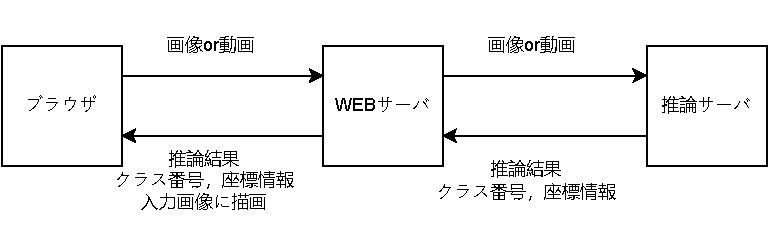
\includegraphics[width=\linewidth]{obj/system.pdf}
	\figcap{システム概要図}{System structure}{OBJ_SYS}
\end{figure}

\section{判別モデルの開発の流れ}
電車が写っている画像を集めて,データセットを作成し,学習をするという流れで判別モデルを開発する.

\subsection{データ収集}
	YouTubeで特定の電車のみが映っている1〜3種類の動画を保存して,電車が映っている場面だけを画像として保存する.
	各車両タイプが名前になっているディレクトリに保存する.
	
\subsection{データセットの作成}
本プロジェクトで作成するモデルは識別モデル,分類モデルの二種類である.データセットのディレクトリ構造が識別用と分類用で異なるので,それぞれのデータセットを作成した.識別モデルには画像のアノテーション情報も必要なので,アノテーションを行い,識別モデル用のデータセットを作成した.
\subsubsection{分類とは}
%画像には何が写っているのかを判断することを分類という.一枚の画像に一つの物体が写っている場合に分類ができる.
分類はデータやオブジェクトを異なるクラスやカテゴリに分けるプロセスを指す.画像の分類とは,画像が特定のカテゴリやクラスに属するかどうかを判別する作業である.例えば,画像に写っているのが猫か犬か,車か飛行機かなどのクラスに分類することがある.
\subsubsection{識別とは}
識別とは画像のどこに何が写っているのかを判断するプロセスを指す.1枚の画像に複数の物体が写っていても識別はできる.

\subsubsection{アノテーションとは}
https://www.dir.co.jp/world/entry/solution/annotation
アノテーションとは、機械学習の分類の一つである教師あり学習において,分析対象データにラベルを付与するプロセスである.画像にバウンディングボックスと呼ばれる四角形を描画しクラス番号を指定する.バウンディングボックスを描画することでその画像に写っている物体の座標情報を取得することができる.クラス番号とは,判別したいものリストを作成し,画像に写っている物体に対応した,リストのインデックスのことである.アノテーションをした結果は,識別モデルの学習時に使用する.
%\subsubsection{分類モデル}
%分類モデルのデータセットは,分類したいものの画像をそれぞれの車両タイプの名前のディレクトリに保存する.

%\subsubsection{識別モデル}
%識別モデルのデータセットは,学習用とテスト用の2種類のディレクトリのそれぞれに画像と画像のアノテーション情報が記載されているテキストファイルを保存する.画像ファイルとそのアノテーション情報のテキストファイルはファイル名を統一する必要がある.\\
%どんなふうにアノテーションをしたのか説明が必要?\\
%アノテーション情報には,クラス番号と画像で物体が写っている部分の座標情報が必要である.
%本プロジェクトにおける識別モデルのクラス番号は,リスト形式で識別したい車両タイプを定義した,それぞれの車両タイプのインデックスとした


\subsection{モデルの学習}
本プロジェクトではYOLOv8を用いてモデルを作成した
\subsubsection{YOLOv8の概要}
YOLOの説明 =>
YOLOとはYou Only Look Onceの略で,人間のように一目見るだけで物体検出ができることを指している.データセットを作成し学習させることで,任意の物体のみ検出させることが可能である.\\
YOLOv8の説明  => 
YOLOv8はYOLOシリーズの最新バージョンであり,ディープラーニングとコンピュータビジョンの最先端の進歩に基づいており,速度と精度の麺で比類のない性能を提供している.
%https://docs.ultralytics.com/ja/ 参照


\subsubsection{学習の実行}
分類・JRではデータセットの画質によって結果が変わるのか,複数のデータセットを作成して学習を行った.\\

\section{作成したモデルについて}
\subsection{モデルの性能評価指標}
本プロジェクトで作成するモデルは混合行列から性能の評価を行う.混合行列とは
	実際のデータと予測データを比較するためのもので,正しくラベル設定ができているのか,及び予測の精確度を把握することができる.
\subsection{分類モデルの性能評価}
適当な図を貼り付ける
\subsection{識別モデルの性能評価}
適当な図を貼り付ける

\subsection{モデルの使い方}
識別モデルと分類モデルをどのように使えば結果が出力されるのかを説明する.pythonのコードを貼り付ける?

\section{考察}
正解率は電車によって異なることがわかる.特に外見が似ている電車だと,誤判別していることが多かった.データセットの画質を落とすと誤判別が増えた.特に誤分類が多かった三種類の電車の画質を上げても結果はあまり変わらなかった.

限られたストレージでは,データセットの画質を変化させて判別結果を向上させることは難しいと考えられる.SSDの容量に制限がない場合,大量の高画質のデータでデータセットを作成することで判別結果が改善される可能性があると考えられる.



\section{文章の書き方}
\subsection{図表の書き方,相互参照}
核融合の仕組みを図\ref{FIG_KUJIRA}に示す\cite{jp2k1,bk1}.核融合の仕組みを図\ref{FIG_CAT}に示す.表\ref{TBL_XYZ},表\ref{TBL_XXX}及び表\ref{TAB_ALPHA}は今年食べて美味しかった果物を示したものである\cite{sdkguide}.

%%%%%%%%%%%%%%%%%%%%%%%%%%%%%%%%%%%%%
\begin{figure} % 小さな図
	\centering
	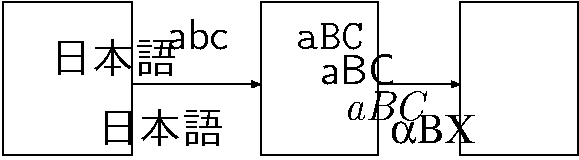
\includegraphics[width=\linewidth]{fig/concept.pdf}
	\figcap{ここに日本語で図題を書く}{Write a figure-caption here in English}{FIG_KUJIRA}
\end{figure}

%%%%%%%%%%%%%%%%%%%%%%%%%%%%%%%%%%%%%
\begin{table} % 小さな表
	\centering
	% \tabcolsep = 10pt % セルごとの左右の余白を削減するときはここで調整
	\tabcap{ここに日本語で表題を書く}{Write a table-caption here in English}{TBL_XYZ}
	\begin{tabular}{lll}
		\Hline
			なまえ & 味 & 産地\\
		\hline
				リンゴ & 92.1 & 青森\\
				みかん & 92.6 & 愛媛\\
				いちご & 90.3 & 金沢\\
		\Hline
	\end{tabular}
\end{table}

%%%%%%%%%%%%%%%%%%%%%%%%%%%%%%%%%%%%%
\begin{table} % 小さな表
	\centering		

	\tabcap{ここに日本語で表題を書く}{Write a table-caption here in English}{TBL_XXX}
	\begin{tabular}{p{5\zw}p{10\zw}}
		\Hline
		名前 & 備考\\
		\hline
		かごめ & どうにもなりません\\
		ききょう & これまたどういうことでありましょう\\
		つばき & さようなら \\
		\Hline
	\end{tabular}
\end{table}

%%%%%%%%%%%%%%%%%%%%%%%%%%%%%%%%%%%%%
\begin{figure*} % 大きな図(二段ぬき)
	\centering
	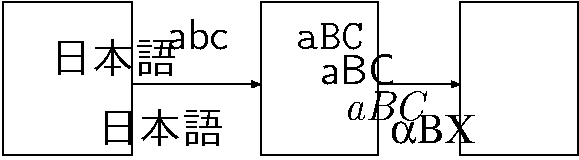
\includegraphics[height=2cm,width=\linewidth]{fig/concept.pdf}
\figcap{二段抜きの大きな図ここに日本語で図題を書く}{Write a figure-caption here in English}{FIG_CAT}
\end{figure*}

%%%%%%%%%%%%%%%%%%%%%%%%%%%%%%%%%%%%%
\begin{table*} % 大きな表(二段ぬき)
	\centering
\tabcap{ここに日本語で表題を書く}{Write a table-caption here in English}{TAB_ALPHA}
	\begin{tabular}{lll}
		\Hline
			なまえ & 味 & 産地\\
		\hline
			おおきなおおきなおおきなおおきなおおきなおおきなおおきなおおきなリンゴ & 92.1000000000 & 青森\\
			おおきなおおきなおおきなおおきなおおきなおおきなおおきなおおきなみかん & 92.6000000000 & 愛媛\\
			おおきなおおきなおおきなおおきなおおきなおおきなおおきなおおきないちご & 90.3000000000 & 金沢\\
		\Hline
	\end{tabular}
\end{table*}
%%%%%%%%%%%%%%%%%%%%%%%%%%%%%%%%%%%%%

\subsection{箇条書き}
あああああああああああああ
\subsubsection{番号付き箇条書き}
番号付きの場合は以下のようにする.番号付きの場合は以下のようにする.番号付きの場合は以下のようにする.
\begin{enumerate}
 \item あああああああ
\item いいいいいいい
\item うううううう
\item ええええええ
\end{enumerate}
ああああああああああああああああああああああああああああああああああああああああああああああああああああああああああああああああああああああ
\subsubsection{見出し付き箇条書き}
見出し付きの場合は以下のようにする.
\begin{description}
 \item[あああああああ]おおおおおおおおおおおお
 \item[いいいいいいい]いいいいいいいいいいいいい
 \item[うううううう]うううううううううううううううううううううううううううううううううううううううううううううううううううううううううううう
 \item[ええええええ]ああああああああああああああああああああああああああああああああああああああああああああああああああああああああ
\end{description}



\section{システム構成}
	あいうえおかきくけこさしすせそたちつてとなにぬねのはひふへほまみむめもやゆよらりるれろわをん.あいうえおかきくけこさしすせそたちつてとなにぬねのはひふへほまみむめもやゆよらりるれろわをん.あいうえおかきくけこさしすせそたちつてとなにぬねのはひふへほまみむめもやよむめもやゆよらりるれろわをん.あいつてとなにぬねのはひふへほまみむめもやゆよらりるれろわをつてとなにぬねのはひふへほまみむめもやゆよらりるれろわをん.あいうえおかきくけこのはひふへほまみむめもやゆよらりるれん.あいうえおかきくけこのはひふへほまみむめもやゆよらりるれろわをん.けこさしすせそたちつてとなにぬねのはひふへほまみむめもやゆよらりるれろわをん.あいうえおかきくけこさしすせそたちつてとなにぬねのはひふへほまみむめもやゆよらりるれろわをん.あいうえおかきくけこのはひふろわをん.けこさしすせそたちつてとなにぬねのはひふへほまみむめもやゆよらりるれろわをん.あいうえおかきくけこさしすせそたちつてとなにぬねのはひふへほまみむめもやゆよらりるれろわをん.あいうえおかきくけこのよらりるれろわをん.あいうえおかきくけこさしすせそたちつてとなにぬねのはひふへほまみむめもやゆよらりるれろわをん.あいうえおかきくけこのはひふへほまみ
	\section{評価実験の方法}
	あいうえおかきくけこさしすせそたちつてとなにぬねのはひふへほまみむめもやゆよらりるれろわをん.あいうえおかきくけこさしせそたちつ

	
		\section{実験結果}
	あいうえおかきくけこさしすせそたちつてとなにぬねのはひふへほまみむめもやゆよらりるれろわをん.あいうえおかきくけこさしすせそたちつてとなにぬねのはひふへほまみむめもやゆよらりるれろわをん.あいうえおかきくけこさしすせそたちつてとなにぬねのはひふへほま	
	\section{考察}
		あいうえおかきくけこさしすせそたちつてとなにぬねのはひふへほまみむめもやゆよらりるれろわをん.あいうえおかきくけこさしすせそたちつてとなにぬねのはひふへほまみむめもやゆよらりるれろわをん.あいうえおかきくけこさしすせそたちつてとなにぬねのはひふへほまみむめもやゆよらりるれろわをん.
	\section{まとめ}
		あいうえおかきくけこさしすせそたちつてとなにぬねのはひふへほまみむめもやゆよらりるれろわをん.あいうえおかきくけこさしすせそたちつてとなにぬねのはひふへほまみむめもやゆよらりるれろわをん.るれろわをん.あいうえおかきくけこさしすせそたちつてとなにぬねのはひふへほまみむめもやゆよらりるれろわをん.

%% 参考文献(必要に応じて追加)
\begin{thebibliography}{99}
\bibitem{jp2k1} 織田 信長, 明智 光秀, "JPEG2000画像符号化システムにおける係数ビットモデリングと適応算術符号化,"Journal of signal processing(基礎シリーズ), vol.7, no.4, pp.257-266, July 2003.
\bibitem{sdkguide}Parrot, "AR.Drone Developer Guide SDK 2.0"
\bibitem{bk1} "金沢の暮らし", \url{http://www.kanazawa-it.ac.jp}
\bibitem{bk2} 山田 太郎, "金沢の一人暮らし", トンチンカン出版, 2016.
\end{thebibliography}

\noindent\textbf{本プロジェクトに関する業績} % 学部
% \noindent\textbf{本研究に関する業績} % 院生の場合
\begin{enumerate}[label=\arabic*),leftmargin=2.25\zw]
\item 鈴木 大志 , 鷹合 大輔 , 中沢 実,"AutoVCを用いたゼロショットリアルタイム声質変換手法の提案",2021-DPS-189(5), 1-6 (2021-12-13) , 2188-8906.
\end{enumerate}

% 本文ここまで ------------------------------------------------------------------
\end{multicols*} 
\end{document}

